	%-=-=-=-=-=-=-=-=-=-=-=-=-=-=-=-=-=-=-=-=-=-=-=-=
%
%        LOADING DOCUMENT
%
%-=-=-=-=-=-=-=-=-=-=-=-=-=-=-=-=-=-=-=-=-=-=-=-=

\documentclass[newPxFont,pagenumber]{beamer}
\usetheme{sthlm}
%\usecolortheme{sthlmv42}

%-=-=-=-=-=-=-=-=-=-=-=-=-=-=-=-=-=-=-=-=-=-=-=-=
%        LOADING PACKAGES
%-=-=-=-=-=-=-=-=-=-=-=-=-=-=-=-=-=-=-=-=-=-=-=-=
\usepackage[utf8]{inputenc}
\usepackage[frenchb]{babel}
\usepackage[normalem]{ulem}
\usepackage{caption}
\captionsetup{font=scriptsize}
%\usepackage[font=footnotesize]{subcaption}
% in preamble
\usepackage{chronology}
\usepackage{pgf}
\usepackage[linesnumbered,ruled,vlined]{algorithm2e}
\usepackage{tikz}
\usetikzlibrary{arrows,automata}
\usepackage{array,multirow}
\usepackage{nameref}
\usepackage{listings}
\usepackage{eurosym}
\usepackage{xcolor}
\definecolor{shadecolor}{RGB}{51,51,51}
\definecolor{darkblue}{rgb}{0.0,0.0,0.6}

\makeatletter
\newcommand*{\currentname}{\@currentlabelname}
\makeatother

\graphicspath{ {fig/} }
% add page number
%\usepackage[defaultsans]{cantarell}

\newcommand{\p}{\mathbb{P}}

\setbeamerfont{title}{series=\upshape}
\setbeamertemplate{footline}{\hfill\footnotesize\insertframenumber\hskip3pt\null\vskip3pt}

\newcommand{\argmax}{\mathop{\mathrm{argmax}}\limits}
\renewcommand{\max}{\mathop{\mathrm{max}}\limits}

\renewcommand{\event}[3][e]{%
  \pgfmathsetlength\xstop{(#2-\theyearstart)*\unit}%
  \ifx #1e%
    \draw[fill=black,draw=none,opacity=0.5]%
      (\xstop, 0) circle (.2\unit)%
      node[opacity=1,rotate=45,right=.2\unit] {#3};%
  \else%
    \pgfmathsetlength\xstart{(#1-\theyearstart)*\unit}%
    \draw[fill=black,draw=none,opacity=0.5,rounded corners=.1\unit]%
      (\xstart,-.1\unit) rectangle%
      node[opacity=1,rotate=45,right=.2\unit] {#3} (\xstop,.1\unit);%
  \fi}%

\addto\captionsfrench{%
\renewcommand{\figurename}{\scriptsize {\scshape Figure}}
\renewcommand{\tablename}{\scriptsize {\scshape Table}}
}

\lstset{
	basicstyle=\tiny,
	breaklines=true,
	showstringspaces=false,
	inputencoding=utf8,
	extendedchars=false,
	literate=% {à}{{\`a}}1 {â}{{\^a}}1 {é}{{\'e}}1 {è}{{\`e}}1 {ê}{{\^e}}1 {î}{{\^i}}1 {ô}{{\^o}}1 {ù}{{\`u}}1 {û}{{\^u}}1 { ̧c}{{\c{}c}}1
	{á}{{\'a}}1 {é}{{\'e}}1 {í}{{\'i}}1 {ó}{{\'o}}1 {ú}{{\'u}}1
	{Á}{{\'A}}1 {É}{{\'E}}1 {Í}{{\'I}}1 {Ó}{{\'O}}1 {Ú}{{\'U}}1
	{à}{{\`a}}1 {è}{{\`e}}1 {ì}{{\`i}}1 {ò}{{\`o}}1 {ù}{{\`u}}1    
	{À}{{\`A}}1 {È}{{\'E}}1 {Ì}{{\`I}}1 {Ò}{{\`O}}1 {Ù}{{\`U}}1
	{ä}{{\"a}}1 {ë}{{\"e}}1 {ï}{{\"i}}1 {ö}{{\"o}}1 {ü}{{\"u}}1
	{Ä}{{\"A}}1 {Ë}{{\"E}}1 {Ï}{{\"I}}1 {Ö}{{\"O}}1 {Ü}{{\"U}}1
	{â}{{\^a}}1 {ê}{{\^e}}1 {î}{{\^i}}1 {ô}{{\^o}}1 {û}{{\^u}}1
	{Â}{{\^A}}1 {Ê}{{\^E}}1 {Î}{{\^I}}1 {Ô}{{\^O}}1 {Û}{{\^U}}1
	{Ã}{{\~A}}1 {ã}{{\~a}}1 {Õ}{{\~O}}1 {õ}{{\~o}}1
	{œ}{{\oe}}1 {Œ}{{\OE}}1 {æ}{{\ae}}1 {Æ}{{\AE}}1 {ß}{{\ss}}1
	{ű}{{\H{u}}}1 {Ű}{{\H{U}}}1 {ő}{{\H{o}}}1 {Ő}{{\H{O}}}1
	{ç}{{\c c}}1 {Ç}{{\c C}}1 {ø}{{\o}}1 {å}{{\r a}}1 {Å}{{\r A}}1
	{€}{{\euro}}1 {£}{{\pounds}}1 {«}{{\guillemotleft}}1
	{»}{{\guillemotright}}1 {ñ}{{\~n}}1 {Ñ}{{\~N}}1 {¿}{{?`}}1 {°}{{$^\circ$}}1 
}

\lstdefinelanguage{XML}
{
	morestring=[b]",
	morestring=[s]{>}{<},
	morecomment=[s]{<?}{?>},
	numbers=none,
	stringstyle=\color{black},
	identifierstyle=\color{darkblue},
	keywordstyle=\color{cyan},
	morekeywords={xmlns,version,type}% list your attributes here
}
%-=-=-=-=-=-=-=-=-=-=-=-=-=-=-=-=-=-=-=-=-=-=-=-=
%        BEAMER OPTIONS
%-=-=-=-=-=-=-=-=-=-=-=-=-=-=-=-=-=-=-=-=-=-=-=-=

%\setbeameroption{show notes}

%-=-=-=-=-=-=-=-=-=-=-=-=-=-=-=-=-=-=-=-=-=-=-=-=
%
%	PRESENTATION INFORMATION
%
%-=-=-=-=-=-=-=-=-=-=-=-=-=-=-=-=-=-=-=-=-=-=-=-=

\title{\large Méthodes D'Analyse Sémantique De Corpus De Décisions Jurisprudentielles}
\subtitle{\scriptsize Soutenance de thèse de doctorat en informatique de l'IMT Mines Alès}
%\date{\small{\jobname}}
%\date{\scriptsize Début de thèse: 15 Décembre 2015}
\date{\scriptsize 24 janvier 2020}
\author{\small Gildas TAGNY NGOMPÉ}
\institute{\tiny \textbf{Jury:} \begin{itemize}
\item Stéphane MUSSARD, Professeur, Université de Nîmes (Directeur de thèse)
\item Jacky MONTMAIN, Professeur, IMT Mines Alès (Co-directeur de thèse)
\item Sandra BRINGAY, Professeur, Université Paul Valéry Montpellier (Rapporteur)
\item Mohand BOUGHANEM, Professeur, Université Toulouse III Paul Sabatier (Rapporteur)
\item Françoise SEYTE, Maître de Conférences (HDR), Université de Montpellier (Examinateur)
\item Fabrice MUHLENBACH,  Maître de Conférences, Université Jean Monnet de Saint-Étienne (Examinateur)
\item Guillaume ZAMBRANO, Maître de Conférences, Université de Nîmes (Encadrant de proximité)
\item Sébastien HARISPE,  Maître Assistant, IMT Mines Alès (Encadrant de proximité)
\end{itemize}}

\hypersetup{
pdfauthor = {\author{}: tagnyngompe@gmail.com},
pdfsubject = {},
pdfkeywords = {},
pdfmoddate= {D:\pdfdate},
pdfcreator = {}
}

\begin{document}
\nocite{}
%-=-=-=-=-=-=-=-=-=-=-=-=-=-=-=-=-=-=-=-=-=-=-=-=
%
%	TITLE PAGE
%
%-=-=-=-=-=-=-=-=-=-=-=-=-=-=-=-=-=-=-=-=-=-=-=-=
\begin{frame}[plain]
	\titlepage
\end{frame}
%}
%-=-=-=-=-=-=-=-=-=-=-=-=-=-=-=-=-=-=-=-=-=-=-=-=
%
%	TABLE OF CONTENTS: Plan
%
%-=-=-=-=-=-=-=-=-=-=-=-=-=-=-=-=-=-=-=-=-=-=-=-=
\section*{Plan}
\begin{frame}[c]{\currentname}
\tableofcontents[hideallsubsections]
\end{frame}

\section{Introduction}

\begin{frame}[c]{Expression du besoin}
	
	\begin{figure}
		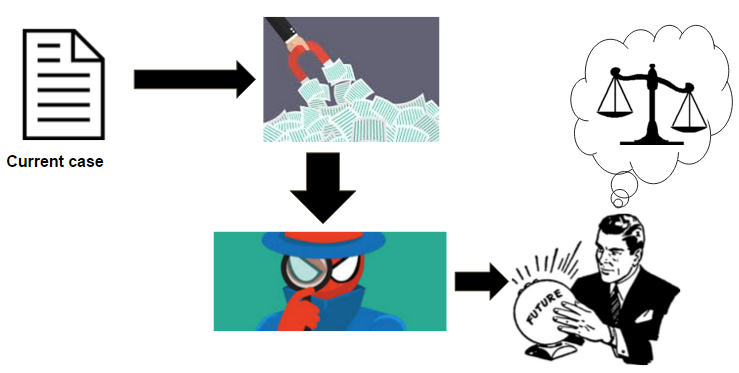
\includegraphics[width=0.7\textwidth]{lawyerwork.png}
		\caption{Les juristes analysent les décisions}
	\end{figure}
	
	\begin{block}{Pourquoi?}
		\begin{itemize}
			\item comprendre et comparer l'application de la loi (contentieux, ville, ...)
			\item estimer le risque judiciaire
			\item ... %anticiper les affaires futures
		\end{itemize}
	\end{block}
\end{frame}

\begin{frame}[c]{Motivation: gros volume de décisions}
	\textbf{Plus de 4 millions de décisions prononcées / an}
	\begin{figure}
		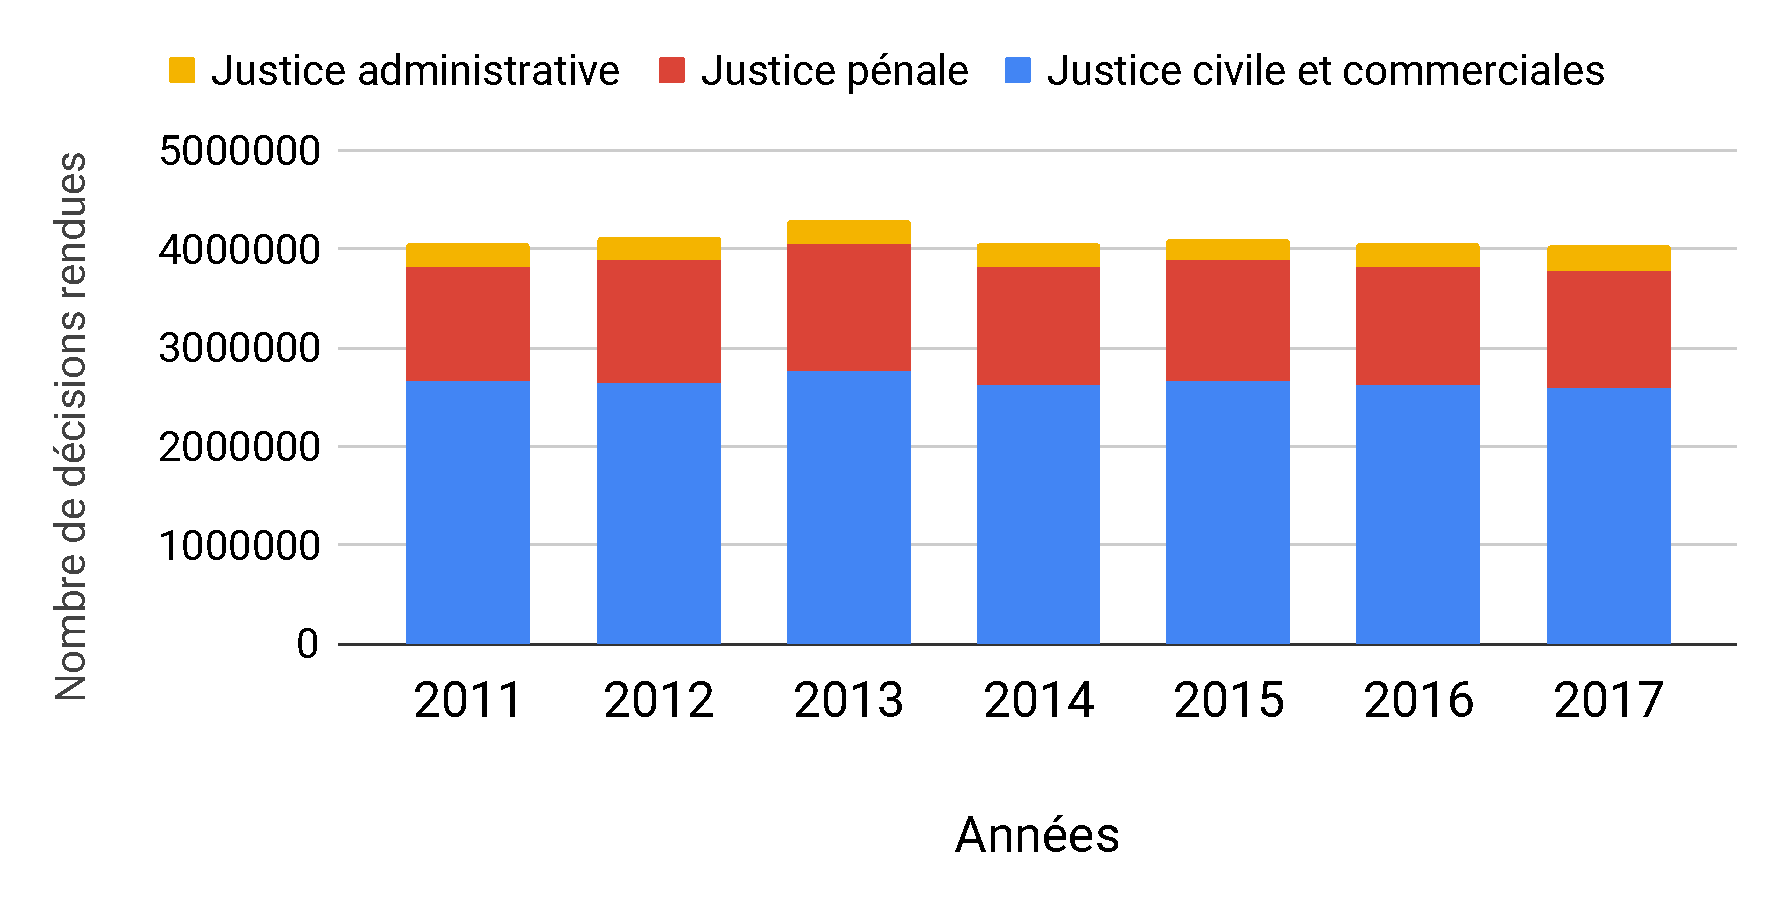
\includegraphics[width=\textwidth]{chiffres-justice.pdf}
		\textit{\tiny{\textbf{Source}: \url{http://www.justice.gouv.fr/statistiques-10054/chiffres-cles-de-la-justice-10303/}}}
		\caption{Nombre de décisions prononcées en France par an de 2011 à 2017.}
	\end{figure}		
\end{frame}

\begin{frame}[t]{Motivation: recherches et analyses sémantiques difficiles}
	
	Moteurs de recherche juridique à mots-clés 
	
	Aucune analyse synthétique des décisions 
	
	\begin{figure}
		\centering
		\fbox{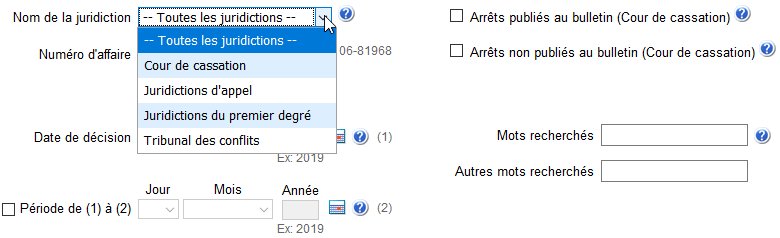
\includegraphics[width=0.9\textwidth]{legifrance.PNG}}
		\caption{Formulaire de Légifrance.}
	\end{figure}
\end{frame}

\begin{frame}[c]{État de l'art : analyse automatique de décisions judiciaires}
	\scriptsize
	\begin{itemize}
		\item Extraction d'information dans les décisions
		\begin{itemize}  \scriptsize
			\item entités juridiques \cite{Waltl2016lexia, andrew2018legalNerAndRelation}
			\item faits \cite{wyner2010extractlegalelts, wyner2010casefactors, Shulayeva2017recognfactprincip}
			\item définitions de concept juridiques \cite{Waltl2016lexia,waltl2017legaliegerman}
			\item arguments \cite{moens2007NBvsMaxent4arguments}
		\end{itemize}
		\item Classification de décisions
		\begin{itemize} \scriptsize
			\item Prédiction des décisions de justice \cite{Ashley2009classifCases, Aletras2016predictDecisionECHR}
			\item identification de la formation et la période \cite{Sulea2017predictareadecision,sulea2017legalEnsSVM}
			\item identifier la sentence prononcée (Chine) \cite{ma2018wmdchinesecase}
		\end{itemize}
		\item Similarité entre décisions 
		\begin{itemize}  \scriptsize
			\item décisions qui citent les mêmes lois et précédents \cite{nair2018judgsimassorule}
			\item recherche d'affaires antérieures pertinentes  \cite{thenmozhi2017legalprecedretriev}
			\item identifier la sentence prononcée (Chine) \cite{ma2018wmdchinesecase}
			\item similarité basée sur la question discutée et les faits sous-jacents (Inde) \cite{kumar2011judgmentsimilarity}
			\item regroupement non-supervisé \cite{raghuveer2012legalclusteringLDA}
		\end{itemize}
	\end{itemize}
\end{frame}

\begin{frame}[c]{Objectif : automatiser des tâches d'analyse de décisions}
%	\only<1>{
		\begin{figure}[!htb]
		% pipeline-cassandra.pdf
		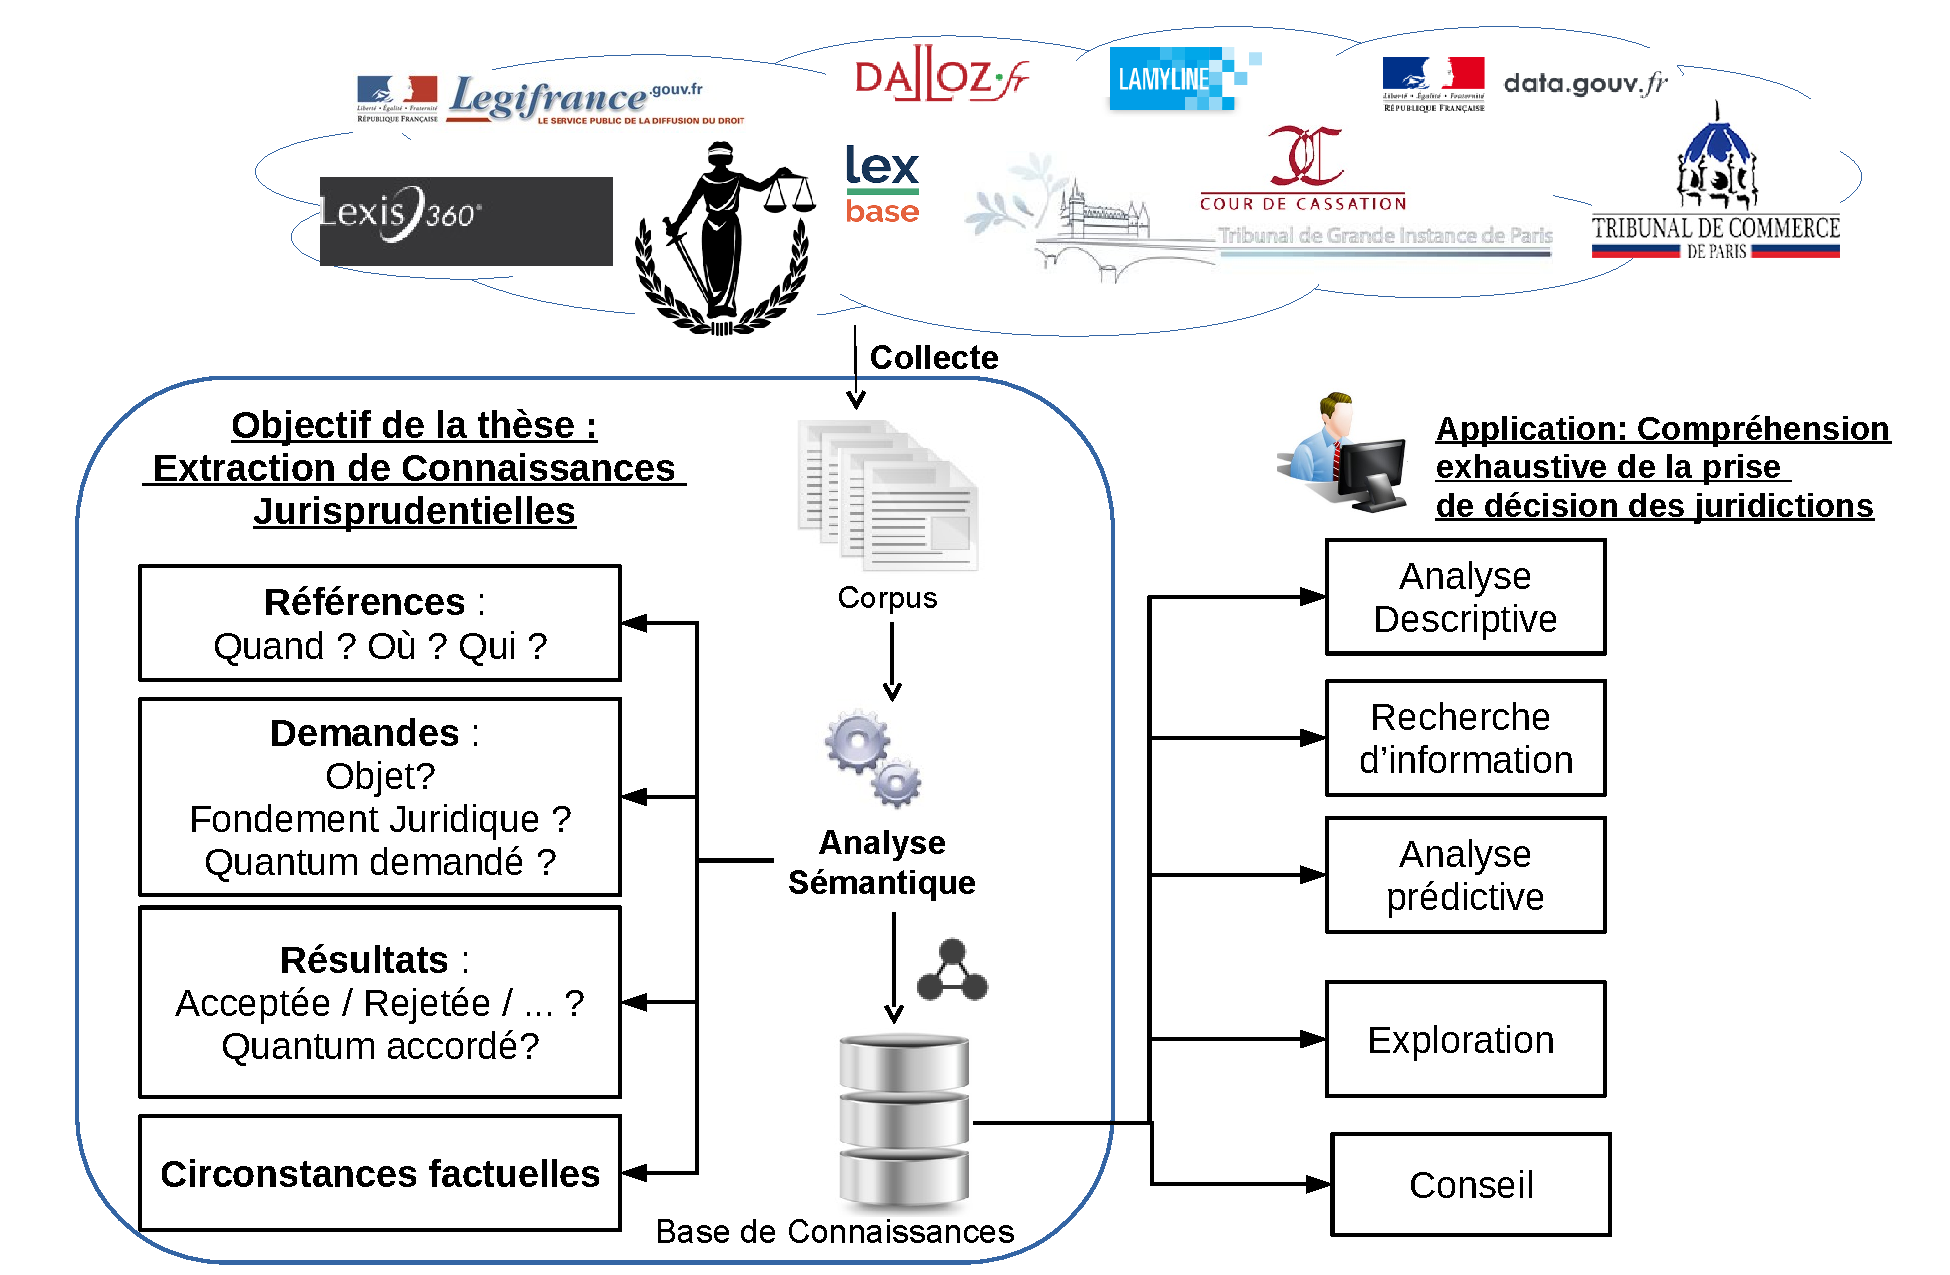
\includegraphics[width=\textwidth]{Objectif_these.pdf}
		\caption{Objectifs et exemples d'application de la thèse.} \label{fig:intro:objectif-these}
	\end{figure}
%}

%	\only<2>{\begin{figure}[!htb]
%		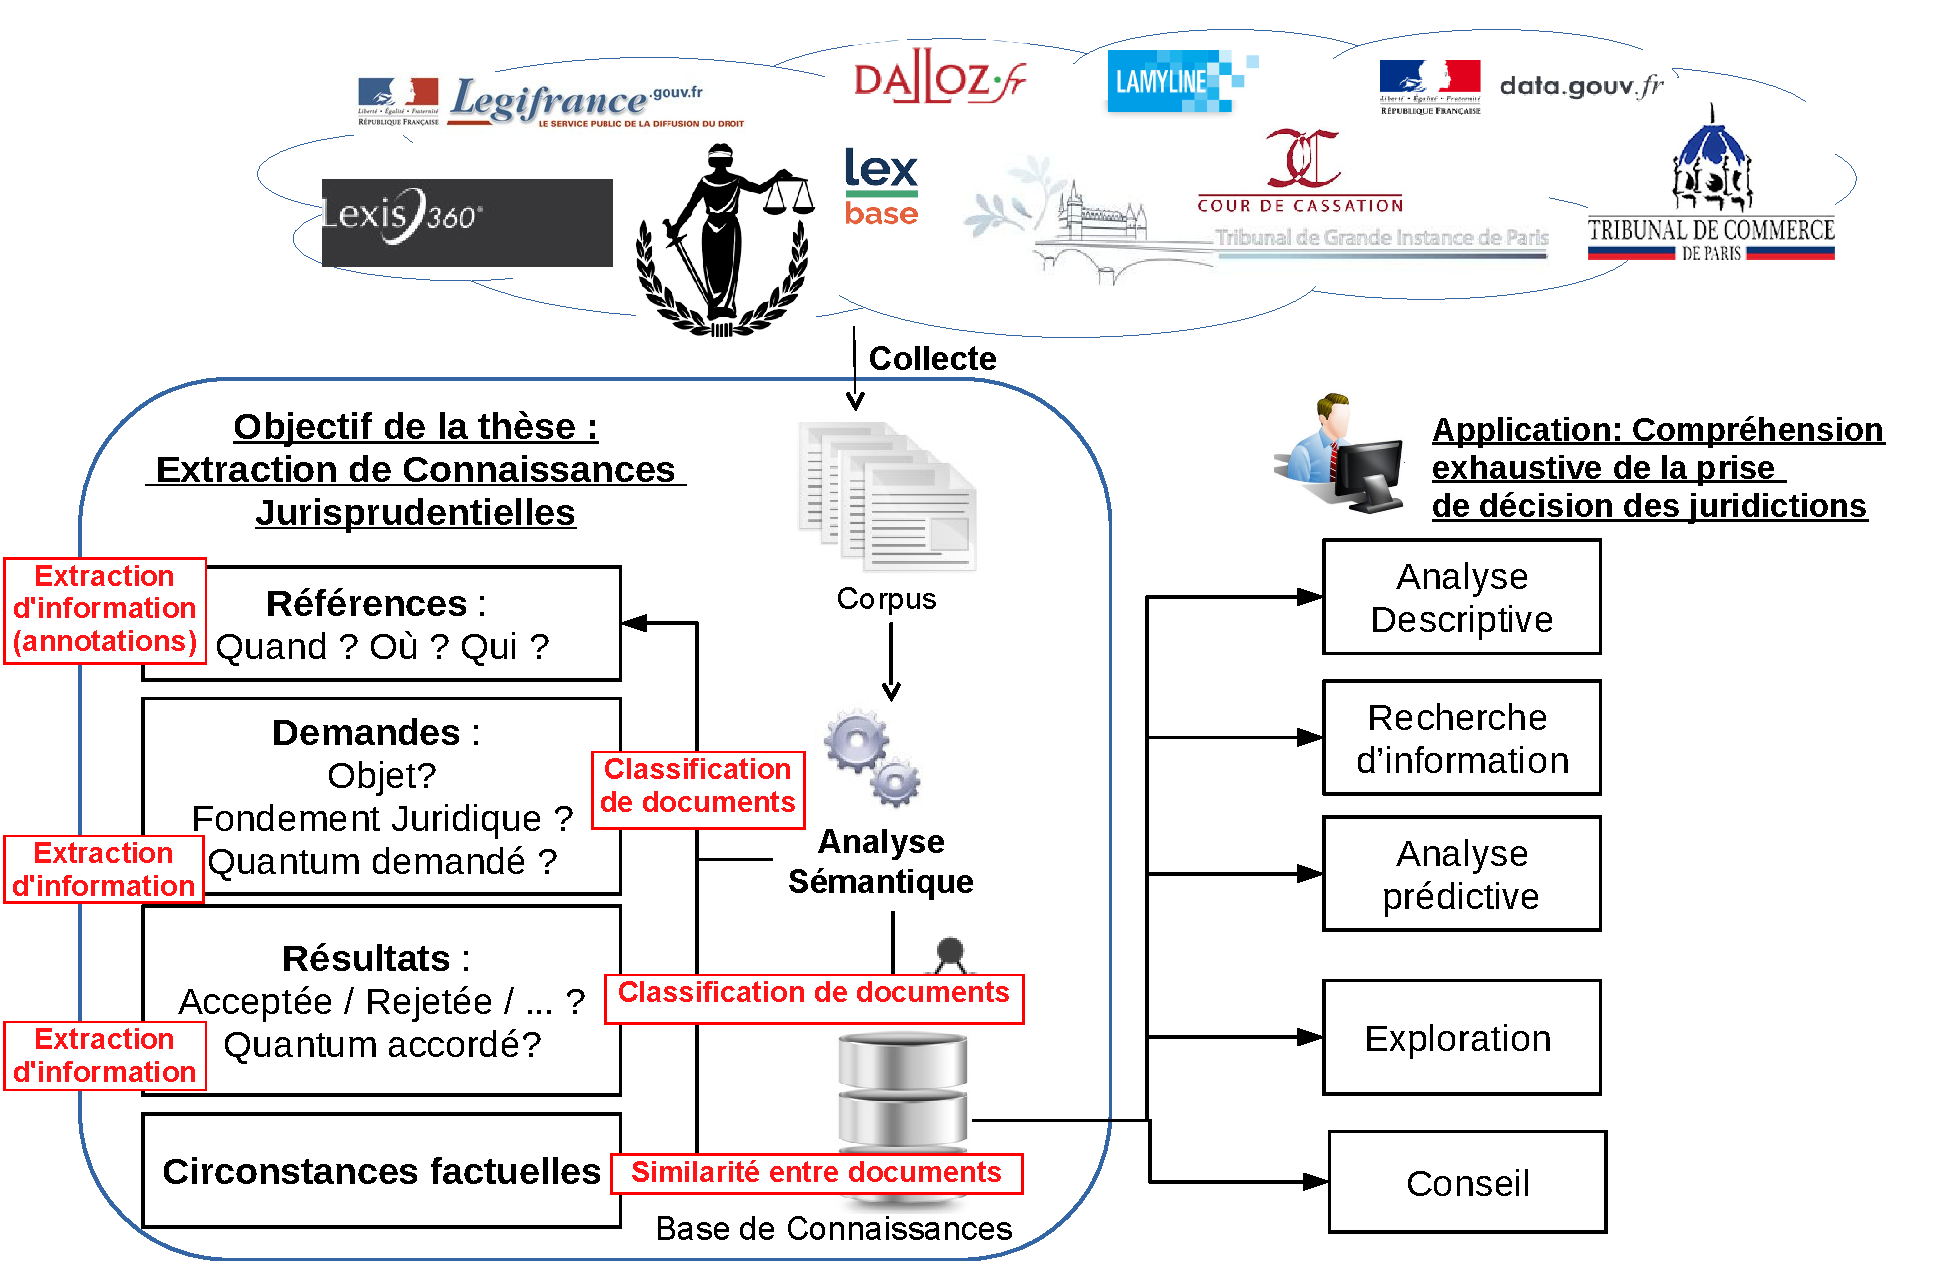
\includegraphics[width=\textwidth]{Objectif_these-problemes2.pdf}
%		\caption{Problèmes correspondants en analyse de données textuelles.} \label{fig:intro:objectif-these-problemes}
%	\end{figure}}
\end{frame}

\begin{frame}[c]{Problème : annotation de sections, métadonnées, normes}
%    \tiny
%	\lstset{language=XMl}
%	\begin{columns}
%		\begin{column}{.50\linewidth}
%        \lstinputlisting{contents/CALYO1406777.xml}
%        \end{column}
%		\begin{column}{.50\linewidth}
%		\lstinputlisting{contents/CALYO1406777-2.xml}
%	    \end{column}
%	\end{columns}
\begin{figure}
	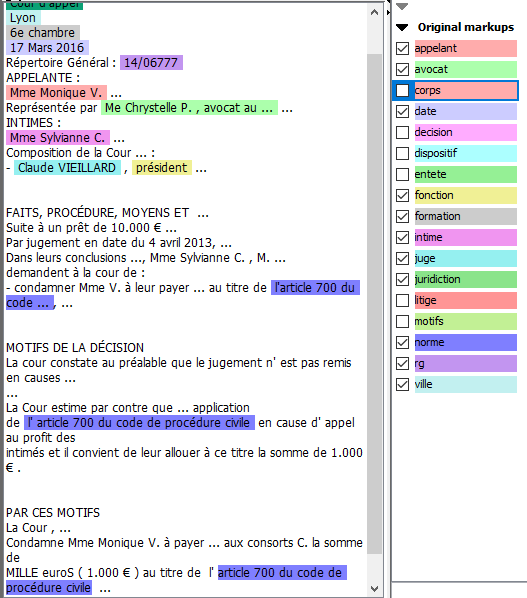
\includegraphics[height=\textheight]{decision-marquee.png}
\end{figure}
\end{frame}

\begin{frame}[c]{Problème : extraction des demandes}
	Cibles : sens du résultat, montant demandé, montant accordé
\begin{exampleblock}{Expression de demande et resultat}
%danais/CASAI1401082.xml
\scriptsize
Jennifer M. et Catherine M. ... demandent à la Cour de :

- \textcolor{orange}{infirmer le dit jugement} en \textcolor{blue}{toutes ses dispositions} ; 
...

Statuant à nouveau ...

- les condamner au paiement d' une somme de  \textbf{3 000,00 € pour procédure abusive} et
aux entiers dépens ; ...

La cour ...  

CONFIRME \textcolor{orange}{le jugement entrepris} en \textcolor{blue}{toutes ses dispositions}.

\end{exampleblock}

\scriptsize{\textit{Légende:  \textcolor{orange}{référence au jugement antérieur},  \textcolor{blue}{agrégation}}}


\begin{table} 
\centering 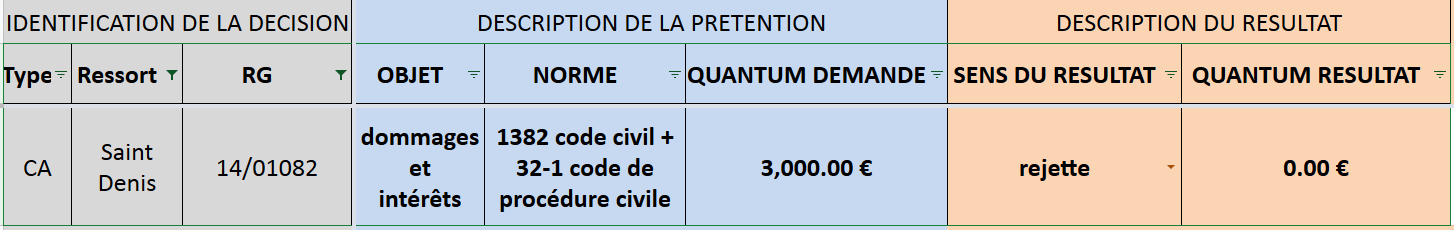
\includegraphics[width=\textwidth]{tab-danais.png}
\caption{\scriptsize Informations à extraire (dommages-intérêts pour procédure abusive)}
\end{table}
\end{frame}

\begin{frame}[c]{Problème : découverte des circonstances factuelles}
  Déterminer les situations distinctes où sont formulées les demandes d'une catégorie données.
    \begin{exampleblock}{Categorie : action en responsabilite civile professionnelle contre les avocats}
	\begin{itemize}
    \item cas $a$ (46 documents): il s'agit d'un avocat négligent qui envoie son assignation de manière tardive ; %(champ sémantique: retard/délai/prescription)
    \item cas $b$ (20 documents): il s'agit d'un avocat qui n'a pas donné un conseil opportun, qui n'a pas soulevé le bon argument;
    \item cas $c$ (18 documents): un avocat qui n'a pas rédigé un acte valide ou réussi à obtenir un avantage fiscal; % (champ sémantique: rédacteur d'actes)
    \item cas $d$ (3 documents): il s'agit d'un avocat attaqué par son adversaire et non par son propre client.
    \end{itemize}
    \end{exampleblock}
\end{frame}

\begin{frame}[c]{Positionnement en fouille de texte}	
	\begin{figure}[!htb]
		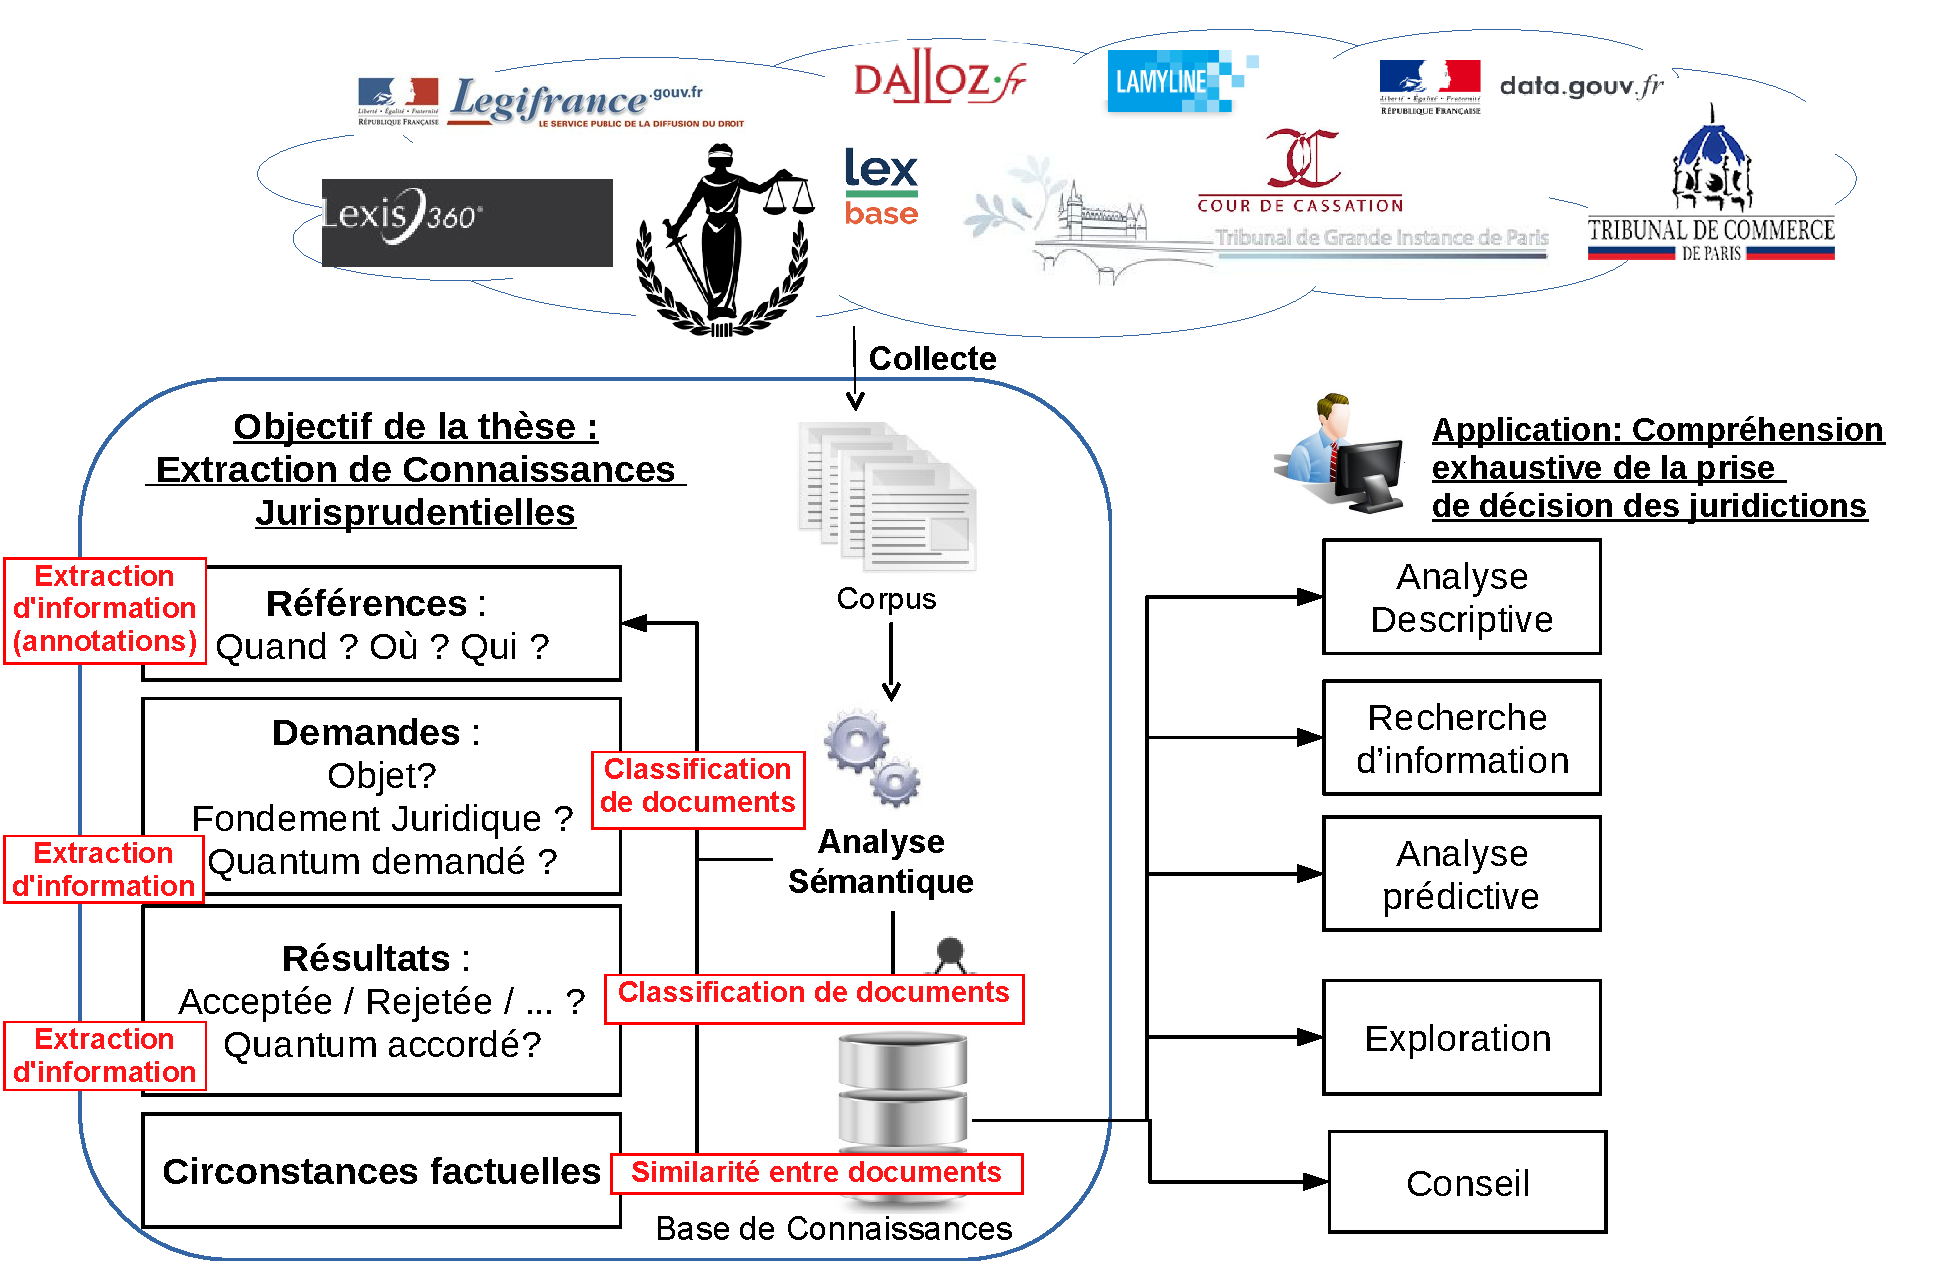
\includegraphics[width=\textwidth]{Objectif_these-problemes2.pdf}
		\caption{Tâches abordées en analyse de données textuelles.} \label{fig:intro:objectif-these-problemes}
	\end{figure}
\end{frame}

\begin{frame}{Difficultés rencontrées par l'automatisation de ces tâches}
	\begin{itemize}
		\item Les décisions sont des textes non-structurés
		\item Le langage juridique est complexe
	\end{itemize}	

	\tiny	
	\begin{columns}
		\begin{column}{.50\linewidth}
			ARRÊT N°
			
			R.G: 11/03924
			
			...
			
			{COUR D'APPEL} DE {NÎMES}
			
			{CHAMBRE CIVILE}
			
			{1ère Chambre A}
			
			ARRÊT DU {20 MARS 2012}
			
			APPELANTE:
			
			{Madame Michéle A.} ...
			
			assistée de la {SELARL VAJOU}, ...
			
			INTIMES:
			
			{Monsieur Martial B} ...
			
			assisté de la {SCP MARION GUIZARD PATRICIA SERVAIS}, ...
			
			COMPOSITION DE LA COUR LORS DU DÉLIBÉRÉ:
			
			{M. Dominique BRUZY, Président}
			
			{M. Serge BERTHET, Conseiller}
			
			...
		\end{column}
		\begin{column}{.50\linewidth}
			FAITS, PROCEDURE, ...
			
			Madame Michèle A. demande:
			
			...
			
			- de condamner Madame JONES-B. à lui payer la somme de {2.500 euros} au titre de l'{article 700 du Code de Procédure Civile}, 
			
			\vspace{0.4cm}
			
			PAR CES MOTIFS, LA COUR:
			
			...
			
			Vu l'{article 809 du Code de Procédure Civile},
			
			...
			
			{Déboute Madame A. de sa demande de provision sur dommages-intérêts.}
			
			...
			
			Vu l'{article 700 du Code de Procédure Civile},
			
			Condamne Madame JONES-B. à verser à Madame A. la somme de {2.500 euros}.
		\end{column}
	\end{columns}
\end{frame}

\section{Analyse automatique des corpus judiciaires}

\begin{frame}[c]{Annotation et extraction d'information}
	
\end{frame}

\begin{frame}[c]{Classification de documents}
	
\end{frame}

\begin{frame}[c]{Similarité entre texte}
	
\end{frame}

\section{Contributions}
\section{Etude des modèles HMM et CRF pour l'annotation des section et entités judiciaires }
\begin{frame}[c]{Appliquer le HMM ou le CRF pour l'annotation}
	\only<1>{1. Méthodes : 	Modèles probabilistes à états et observations

\scriptsize
\begin{table}[]%width=\linewidth
	%\begin{tabular}[]{p{0.40\linewidth}|p{0.55\linewidth}}
	\begin{tabular}[]{c|c}
		\toprule
{\textbf{HMM}} & {\textbf{CRF}} \\
%		\midrule
%		\textbf{Generative} models 	& \multicolumn{2}{c}{"\textbf{Discriminative}" or "\textbf{Conditional}" models } \\[0.25em]
%\midrule		
%"\textbf{generate}" input	& {"\textbf{condition}" on input }\\%[0.25em]
\midrule
{un seul descripteur  par observation}	& {plusieurs descripteurs complexes par observation}\\%[0.25em]
\midrule	
		\begin{tikzpicture}[->,>=stealth',shorten >=1pt,auto,node distance=1.3cm,
                    semithick]
  \node[state] (S1)                    {$s_{t-1}$};
  \node[state]         (S2) [right of=S1] 	  {$s_{t}$};
  \node[state]         (O) [below of=S2] {$o_{t}$};
  \path (S1) edge              node {} (S2)
        (S2) edge              node {} (O);
\end{tikzpicture}
				& 

\begin{tikzpicture}[auto,>=stealth',shorten >=1pt,auto,node distance=1.3cm,
                    semithick]
  \node[state] (S1)                    {$s_{t-1}$};
  \node[state]         (S2) [right of=S1] 	  {$s_{t}$};
  \node[state]         (O) [below of=S2] {$o_{t}$};
  \path (S1) edge              node {} (S2)
        (S2) edge              node {} (O);
\end{tikzpicture}					
					\\%[0.25em]
\midrule
$P_\lambda(S|O) = \prod\limits_{t=1}^{T} P(s_t \vert s_{t-1}) * P(o_t \vert s_{t})$  & $P_\lambda(S|O) = \frac{1}{Z(O)}exp\left( \sum\limits_{t=1}^{T}\sum\limits_{k} \lambda_k f_k(s_{t-1},s_t, o_t) \right) $ \\
% & & & \\
\tiny \cite{Seymore1999hmm} & \tiny \cite{peng2006crf} \\ 
		\bottomrule
	\end{tabular}
\end{table}

\footnotesize

Objectif: Trouver la séquence la plus probable d'étiquetage pour l'ensemble du texte

\textbf{Entrainement fait sur des séquences préalablement étiquetées}
}
	\only<2>{2. Données}
	\only<3>{3. Résultats}	
\end{frame}
\section{Identification des demandes des parties}
\subsection{Objectif de la tâche}
\begin{frame}[c]{\mysubsectiontitle}
Extraction de données sur les demandes des parties
\begin{itemize} \scriptsize 
	\item Exemple : demande de dommage-intérêts pour procédure abusive
	%danais/CASAI1401082.xml
	\begin{itemize} \scriptsize 
		\item Extrait de décision relatif à la demande: 
\fbox{\parbox{0.8\textwidth}{\tiny
	Jennifer M. et Catherine M. ... demandent à la Cour de :
	
	- \textcolor{red}{infirmer le dit jugement} en \textcolor{blue}{toutes ses dispositions} ; 
	...
	
	Statuant à nouveau ...
	
	- les condamner au paiement d'une somme de  \textbf{3 000,00 \euro{} pour procédure abusive} et
	aux entiers dépens ; ...
	
	La cour ... CONFIRME \textcolor{red}{le jugement entrepris} en \textcolor{blue}{toutes ses dispositions}.}}
	\textit{\tiny Légende : référence au jugement antérieur en \textcolor{red}{rouge}, énoncés fusionnés en \textcolor{blue}{bleue}}
    \item Données à extraire       
	\end{itemize}
\end{itemize}
 \centering{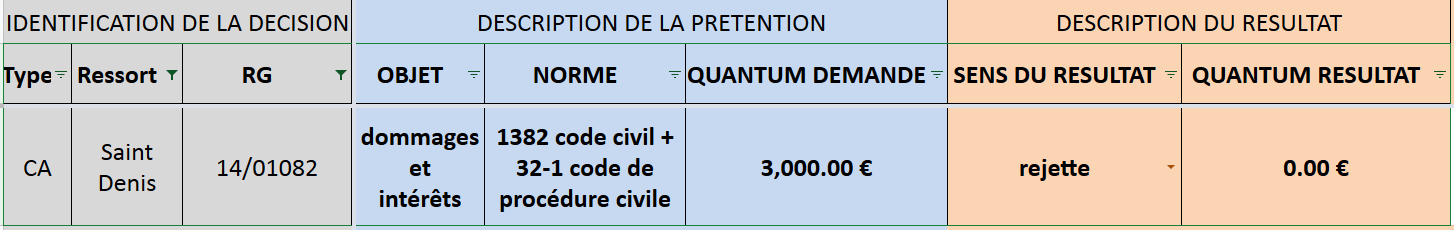
\includegraphics[width=\textwidth]{tab-danais.png}}
 
 \vspace{-0.2cm}
 \begin{itemize} \scriptsize 
\item Difficultés
	\begin{itemize}\scriptsize 
		\item Présence de plusieurs demandes de catégories similaires et/ou différentes dans une même décision
		\item Toutes les catégories ne sont pas connues d'avance (+500 catégories)
		\item Difficile d'annoter une base d'évaluation pour toutes les couvrir
		%\item Énonces non structurés, avec des références, et des agrégations
	\end{itemize}
\end{itemize}
\end{frame}

\subsection{Méthode proposée : approche par catégorie de demandes}

\begin{frame}[t]{\mysubsectiontitle}
	Extraction d'une seule catégorie ($c$) à l'aide de sa terminologie
	
	\begin{itemize} \scriptsize	
		\item Détection de la présence de la catégorie par classification de la décision ($c$ vs. $\overline{c}$)
		%\item Identification des passages de demandes (section Litige) et résultats (section Dispositif)
		\item Identification des quantas : montants à proximité des termes-clés de $c$ dans les énoncés explicites de demandes et résultats		

		\fbox{\parbox{0.8\textwidth}{\scriptsize
				Jennifer M. et Catherine M. ... demandent à la Cour de :
				
				- infirmer le dit jugement en toutes ses dispositions ; 
				...
				
				Statuant à nouveau ...
				
				- \textbf{[} les condamner au paiement d' une somme de  \fbox{\parbox{0.13\textwidth}{\textit{\fontfamily{qcs}\selectfont{3 000,00 \euro}}}}  \textbf{pour procédure abusive} et
				aux entiers dépens ; \textbf{]}$_\text{demande\_danais}$ ...
			
			La cour ... CONFIRME le jugement entrepris en toutes ses dispositions.}}
		
	    \item Identification du sens du résultat 
	    \begin{itemize} \scriptsize
	    	\item soit en fonction du verbe introductif de l'énoncé du résultat	 
	    	\begin{tabular}{|p{0.34\textwidth}|p{0.22\textwidth}|p{0.22\textwidth}|}
	    		\hline
 \multicolumn{3}{|c|}{\textbf{Résultat} (par polarité)} \\ \hline
	    		\textbf{accepte}  &\textbf{sursis à statuer} & \textbf{rejette}  \\ \hline
 \textit{accorde, admet, condamne, ...} & \textit{réserve, surseoit, ...} & \textit{déboute, rejette, ...} \\ \hline
	    	\end{tabular}   	
	    	\item soit \textit{"rejette"} si pas d'énoncé explicite du résultat
	    \end{itemize}
		\item Mise en correspondance des informations relatives à la même demande
		\begin{itemize} \scriptsize
			\item énoncé demande et énoncé résultat similaires
			\item quantum demandé et quantum accordé apparaissant dans le même ordre
		\end{itemize}
	\end{itemize}
\end{frame}

\begin{frame}[t]{\mysubsectiontitle}
	Apprentissage de la catégorie à extraire
	\begin{itemize} \scriptsize
		\item Entraînement d'un algorithme de classification pour détecter sa présence 
		\item Détermination automatique de sa terminologie à l'aide d'une méthode de pondération de termes : 
		\begin{itemize} \scriptsize
			\item $idf(t) = \log_2\left(\frac{N}{N_t}\right)$ \cite{sparck1972idf}
			\item $\Delta_{DF}(t,c) = DF_{t \vert c} - DF_{t \vert \overline{c}}$
			\item $\chi^2(t,c) = \frac{N ((N_{t,c} N_{\overline{t},\overline{c}}) - (N_{t,\overline{c}} N_{\overline{t},c}))^2}{N_t N_{\overline{t}} \vert D_c \vert \vert D_{\overline{c}} \vert }$ \cite{schutze1995chi2}
			\item $ngl(t,c) = \frac{\sqrt{N} (N_{t,c} N_{\overline{t},\overline{c}}) - (N_{t,\overline{c}} N_{\overline{t},c})}{\sqrt{N_t N_{\overline{t}} \vert D_c \vert \vert D_{\overline{c}} \vert }}$ \cite{ng1997ngl}
			\item etc.
		\end{itemize}
	\end{itemize}
\end{frame}
\subsection{Résultats expérimentaux}
\begin{frame}[t]{\mysubsectiontitle}
	Catégories sur lesquelles la méthode a été expérimentée
	
	\scriptsize
		\begin{tabular}{|c|p{0.35\textwidth}|p{0.15\textwidth}|p{0.3\textwidth}|}
			\hline
			\textbf{Label} & \textbf{Nom} & \textbf{Objet} & \textbf{Fondement} \\ \hline
			\textit{acpa} & amende civile pour abus de procédure & amende civile & Articles 32-1 code de procédure civile + 559 code de procédure civile \\ \hline
			\textit{concdel} & dommages-intérêts pour concurrence déloyale & dommages-intérêts & Article 1382 du code civil \\ \hline
			\textit{danais} & dommages-intérêts pour abus de procédure & dommages-intérêts & Articles 32-1 code de procédure civile + 1382 code de procédure civile \\ \hline
			\textit{dcppc} & déclaration de créance au passif de la procédure collective & déclaration de créance & L622-24 code de commerce \\ \hline
			\textit{doris} & dommages-intérêts pour trouble de voisinage & dommages-intérêts & principe de responsabilité pour trouble anormal de voisinage \\ \hline
			\textit{styx} & frais irrépétibles & dommages-intérêts & Article 700 du code de procédure civile \\ \hline
		\end{tabular}
\end{frame}
\begin{frame}[t]{\mysubsectiontitle}
	Quantité de décisions annotées manuellement par l'expert
	
	\centering	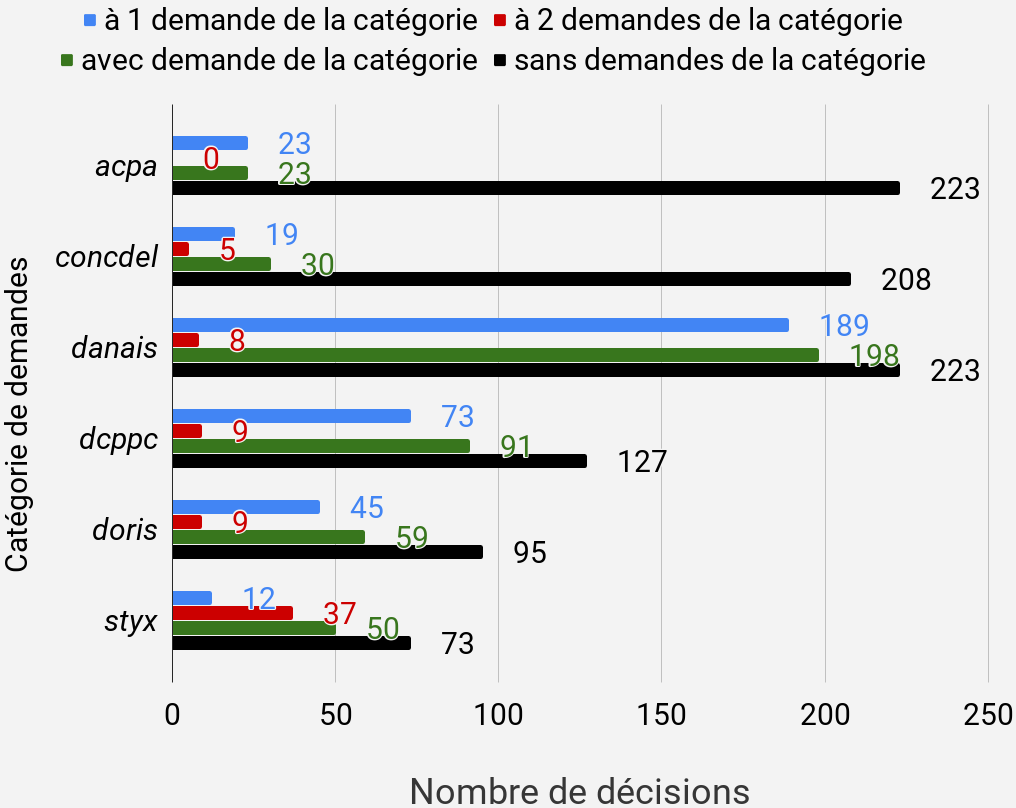
\includegraphics[width=0.8\textwidth]{chartDataset.png}
\end{frame}


\begin{frame}[t]{\mysubsectiontitle}
	Efficacité de la méthode
	\begin{itemize} \scriptsize
		\item Les algorithmes traditionnels (KNN, SVM, naïf bayésien, arbre) donnent de bons résultats pour la détection de la catégorie : $98.8\% \leq F_1 \leq 100\%$
		\item Extraction :
		{\centering{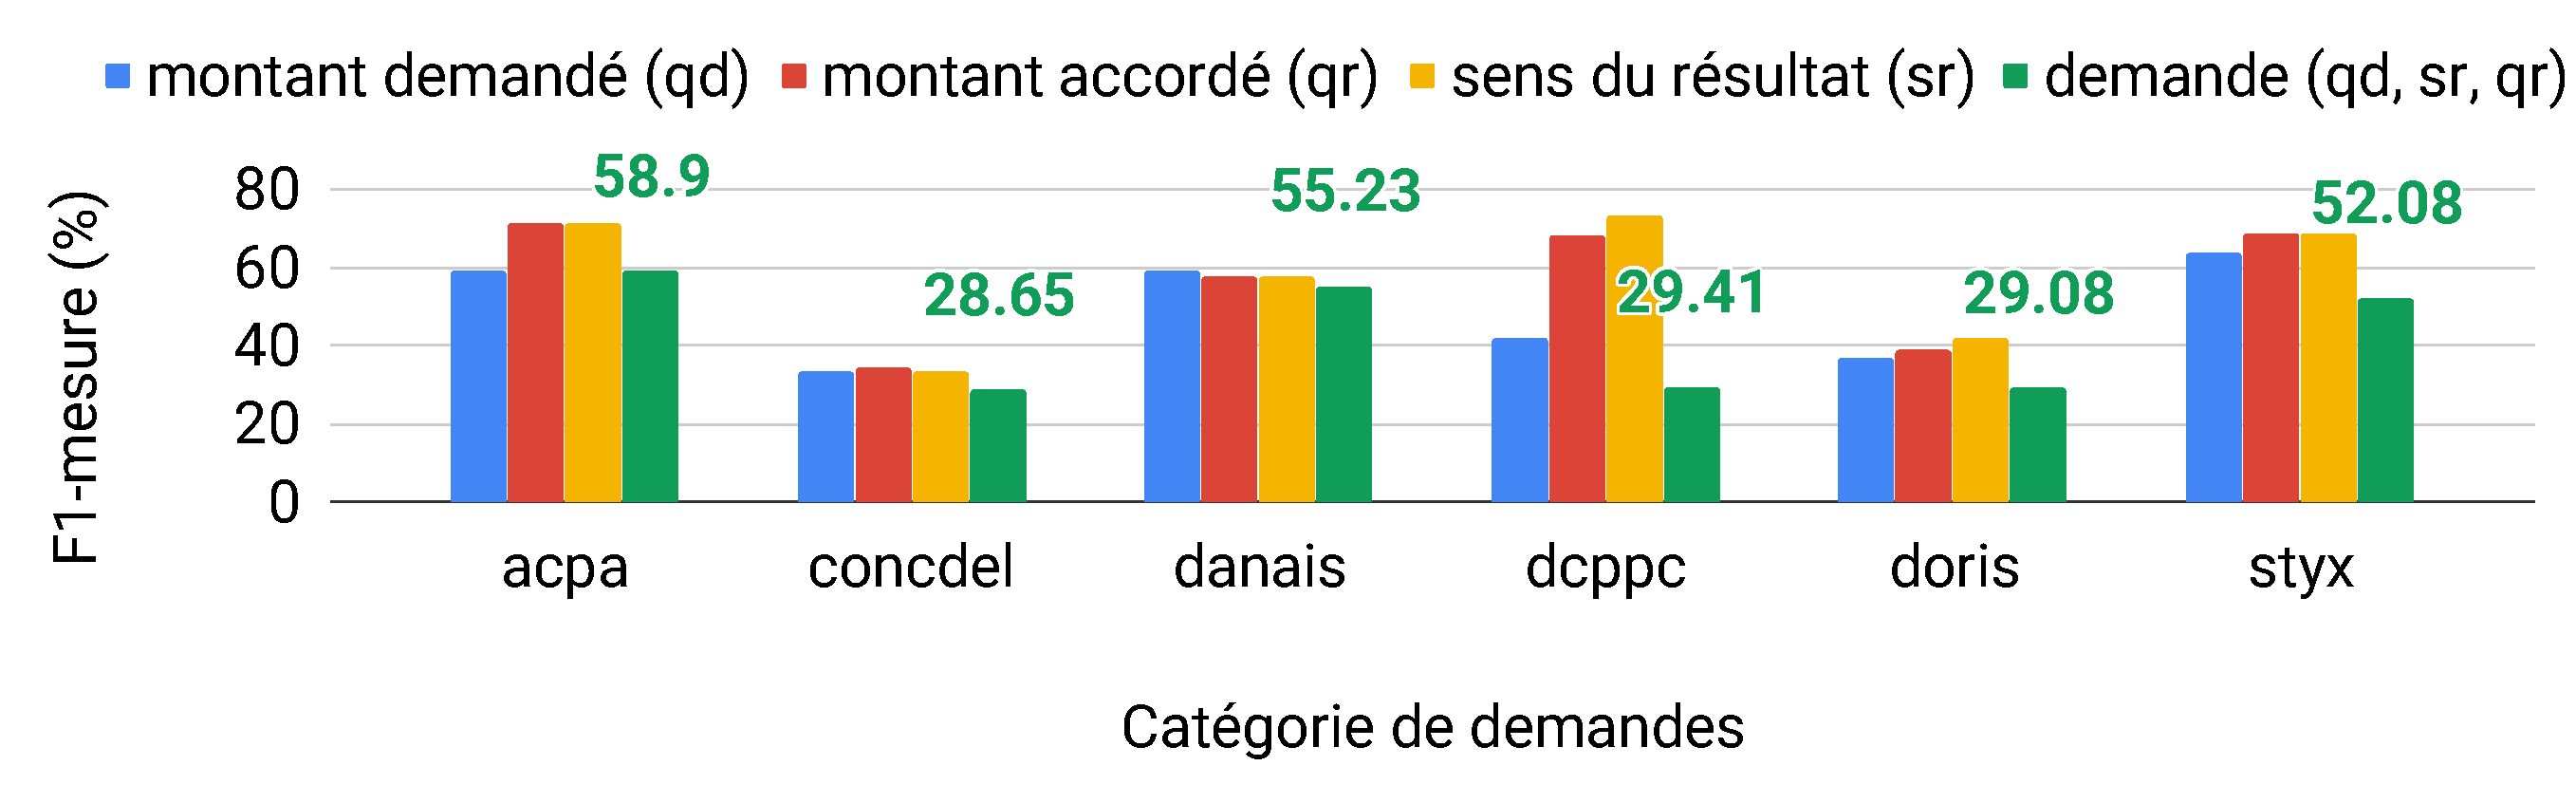
\includegraphics[width=0.9\textwidth]{f1-quanta-et-sens.pdf}}}
		\begin{itemize} \scriptsize
			\item Le résultat est plus accessible 
			\item Certaines catégories (\textit{acpa, danais, styx}) sont plus accessibles que d'autres (\textit{concdel, dcppc, doris})
		\end{itemize}				
		\item Sources d'erreurs:
		\begin{itemize} \scriptsize
			\item Difficulté à identifier les termes-clés rares
			\item Absence de certains quanta dans les énoncés de demandes et résultats
			\item Erreur de mise en correspondance des données extraites
		\end{itemize}
	\end{itemize}
\end{frame}

\section{Identification du sens du résultat}


\subsection{Contexte}

\begin{frame}[t]{\mysubsectiontitle}
	Restriction du problème d'identification des demandes
\begin{itemize}	\small
	\item Uniquement les décisions à une demande de la catégorie
	\begin{itemize}\scriptsize
		\item Raison: plus de $50\%$ des documents dans la majorité des catégories
	\end{itemize}
	\item Classification binaire (éviter les subtilités de rédaction)
	\begin{itemize} \scriptsize
		\item Raison: les demandes sont en majorité \textbf{acceptées} ou \textbf{rejetées}
	\end{itemize}
\end{itemize}
\centering 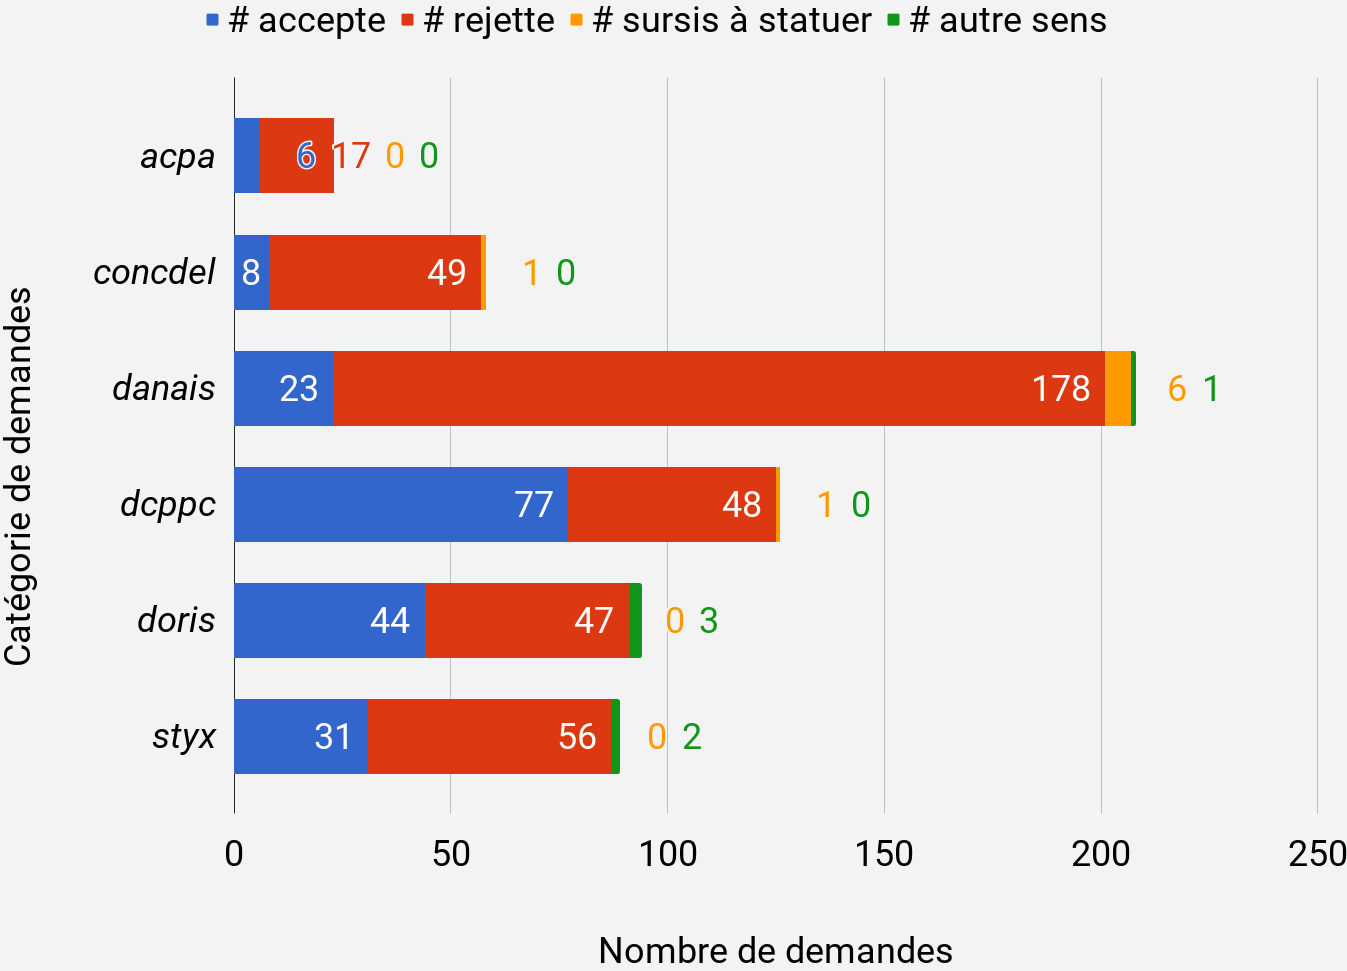
\includegraphics[width=0.7\textwidth]{chartDistrSens.png}
\end{frame}

\begin{frame}[t]{\mysubsectiontitle}
	Plusieurs algorithmes classiques existent
	\begin{itemize} \small
		\item Classifieur bayésien naïf \cite{duda1973patternclass} 
		\item K-plus-proches-voisins \cite{cover1967knn}
		\item SVM \cite{vapnik1995statlearning}
		\item Arbre de décision
		\item Analyse discriminante linéaire \cite{fisher1936linearDA} et quadratique \cite{McLachlan1992DiscrAnalyStatPattRecog-QDA}
		\item Logit-PLS \cite{tenenhaus2005logitpls}
		\item NBSVM \cite{wang2012nbsvm}
		\item fastText \cite{grave2017fasttextcls}
		\item etc.	
	\end{itemize}
\end{frame}


\subsection{Méthodes proposées : adaptations de la régression Gini-PLS}

\begin{frame}[t]{\mysubsectiontitle}
Régression Gini-PLS
\begin{itemize}\small
	\item PLS \cite{wold1966pls} (régression partielle des moindres carrés) 
	\begin{itemize}\scriptsize
		\item Réduction supervisée de dimensions $x_1, x_2, ..., x_m$ en composantes orthogonales $t_1, ...., t_h$
		
		\[t_h = \sum_{k=1}^m w_{hk}\cdot \hat{U}_{(h-1)k}\] 
		
		avec $\hat{U}_{0k} = x_{k}$, $\forall h > 0, \hat{U}_{hk}$ est le résidu de la régression de $x_k$ sur $t_1, ..., t_{h-1}$ 
		
		et $w_{hj} = \frac{\cov(\varepsilon_h, \hat{U}_{(h-1)j})}{\sqrt{\sum_{j=1}^m cov^2(\varepsilon_h, \hat{U}_{(h-1)j})}}$ (solution de $\max \cov(y,w_hX)$ s.c. $\| w_h\|=1$)
		\item Régression de la variable dépendante $y$ dans l'espace réduit
		\[y=c_1 t_1 + ... + c_h t_h + \varepsilon_h\]			
		%\item intérêt : robustesse au problème de haute dimension et élimination du pro
	\end{itemize}
	\item Gini-PLS  \cite{mussard2018ginipls}
	\begin{itemize} \scriptsize
		\item Remplacement de la covariance $\cov(x_j, y)$ par la covariance de Gini $\cog(y; x_j) := \cov(y; R(x_j))$
		\item Élimination de la sensibilité du PLS aux valeurs aberrantes
	\end{itemize}	 	
	
\end{itemize} 
\end{frame}

\begin{frame}[t]{\mysubsectiontitle}
	Algorithmes proposés {\scriptsize (en cours de rédaction pour la revue \textit{\textbf{Stats}})}
\begin{itemize} \small
\setlength\itemsep{1.5em}

\item Gini-PLS généralisé
\begin{itemize} \scriptsize
	\item Utilisation de l'opérateur co-Gini généralisé : \[\cog_\nu(x_\ell,x_k) := -\nu \cov(x_\ell,r_{k}^{\nu-1}) ; \ \nu > 1\] où $r_{k}$ est le vecteur rang décroissant de la variable $x_k$
	
	\item $\nu$ contrôle le compromis entre l'atténuation de la variabilité des variables ($\nu \rightarrow 1$) et l'influence des queues de distributions ($\nu \rightarrow \infty$)	
\end{itemize}

%\item Logit-PLS:  $\forall j > 1$, les $w_{hj} $ sont les coefficients de la régression logistique de $y$ sur les composantes $t_1, ..., t_{h-1}, u_{(h-1)j}$ \cite{tenenhaus2005logitpls}

\item Logit-Gini-PLS  généralisé : 
\begin{itemize} \scriptsize
	\item Estimation des $w_{hj}$ à partir du paramètre $\beta$ de $P(y_i = 1 / X = X_i) = \frac{\exp\left\{X_i \beta \right\}}{1+\exp\left\{ X_i \beta \right\}}$, où $X_i$ étant une observation
	\[w_j = \frac{\beta_j}{\| \beta\|}\]	
	\item les $\hat{U}_{(h)j}$ toujours estimé avec le co-Gini généralisé
\end{itemize} 
\end{itemize}
\end{frame}


\subsection{Résultats expérimentaux}

\begin{frame}[t]{\mysubsectiontitle}
	Comparaison des classifieurs PLS aux classifieurs classiques

	\scriptsize
	\centering
	\begin{tabular}{|l|l|l|l|}
		\hline
		{Représentation} & {Algorithme} & {$F_{1}$} & $F_{1_\text{arbre}} - F_1$  \\ \hline
		
		$tf-gss$ & Arbre & 0.668 & 0\\ \hline
		$tf - avg_{global}$ & LogitPLS & 0.648 & 0.02   \\ \hline
		$tf - avg_{global}$ & StandardPLS & 0.636 & 0.032  \\ \hline
		$tf - \Delta_{DF}$ & GiniPLS & 0.586 & 0.082  \\ \hline
		$tf - \Delta_{DF}$ & GiniLogitPLS & 0.578 & 0.09  \\ \hline
		- & NBSVM & 0.494 & 0.174   \\ \hline
		- & fastText & 0.412 & 0.256  \\ \hline
	\end{tabular}	

\end{frame}

\begin{frame}[t]{\mysubsectiontitle}
	Amélioration de la classification par restriction du document

	\tiny
	\centering
	
	\begin{tabular}{|c|l|l|l|c|}
		\hline
		{Catégorie} & \multicolumn{1}{c|}{Zone} & \multicolumn{1}{c|}{Représentation} & \multicolumn{1}{c|}{Algorithme} & $F_1$ \\ \hline
		\multirow{3}{*}{\textit{acpa}} & \textbf{demande\_resultat\_a\_resultat\_context} & $tf-dbidf$ & \textbf{Arbre} & \textbf{0.846} \\ 
		& litige\_motifs\_dispositif & $tf-dbidf$ & StandardPLS & 0.697 \\ 
		& litige\_motifs\_dispositif & $tf-avg_{global}$ & LogitPLS & 0.683 \\ \hline
		
		\multirow{3}{*}{\textit{concdel}} & \textbf{litige\_motifs\_dispositif} & \textbf{$tf-gss$} & \textbf{Arbre} & \textbf{0.798} \\ 
		& motifs & $tf-idf$ & GiniLogitPLS & 0.703 \\ 
		& context & $logave-dbidf$ & StandardPLS & 0.657 \\ \hline
		
		\multirow{3}{*}{\textit{danais}} & \textbf{demande\_resultat\_a\_resultat\_context} & \textbf{$avg_{local}-\chi^2$} & \textbf{Arbre} & \textbf{0.813} \\ 
		& demande\_resultat\_a\_resultat\_context & $atf-avg_{global}$ & LogitPLS & 0.721 \\ 
		& demande\_resultat\_a\_resultat\_context & $atf-avg_{global}$ & StandardPLS & 0.695 \\ \hline
		
		\multirow{3}{*}{\textit{dcppc}} & \textbf{demande\_resultat\_a\_resultat\_context} & $tf-\chi^2$ & \textbf{Arbre} & \textbf{0.985} \\ 
		& demande\_resultat\_a\_resultat\_context & $tf-\chi^2$& LogitPLS & 0.94 \\ 
		& litige\_motifs\_dispositif & $tp-mar$ & StandardPLS & 0.934 \\ \hline
		
		\multirow{3}{*}{\textit{doris}} & \textbf{litige\_motifs\_dispositif} & $tp-dsidf$ & \textbf{GiniPLS} & \textbf{0.806} \\
		& litige\_motifs\_dispositif & $tp-dsidf$ & GiniLogitPLS & 0.806 \\
		& litige\_motifs\_dispositif & $atf-ig$ & StandardPLS & 0.772 \\ \hline
		
		\multirow{3}{*}{\textit{styx}} & \textbf{motifs} & $tf-dsidf$ & \textbf{Arbre} & \textbf{1} \\ 
		& demande\_resultat\_a\_resultat\_context & $logave-dsidf$ & GiniLogitPLS & 0.917 \\ 
		& litige\_motifs\_dispositif & $tf-rf$& GiniPLS & 0.833 \\ \hline
	\end{tabular}
	
\end{frame}
\section{Découverte des circonstances factuelles}
\subsection{Objectif de la tâche}
\begin{frame}[t]{\mysubsectiontitle}
	Déterminer les situations distinctes où sont formulées les demandes d'une catégorie données
	\begin{itemize} \scriptsize
		\item Exemple : catégorie "action en responsabilité civile professionnelle contre les avocats" (\textit{arcpa})
			\begin{itemize}\scriptsize
				\item cas $a$ : un avocat négligent qui envoie son assignation de manière tardive; 
				\item cas $b$ : un avocat qui n'a pas donné un conseil opportun, qui n'a pas soulevé le bon argument;
				\item cas $c$ : un avocat qui n'a pas rédigé un acte valide ou réussi à obtenir un avantage fiscal; 
				\item cas $d$ : un avocat attaqué par son adversaire et non par son propre client.
			\end{itemize}
		\item Formulation comme un problème de regroupement non supervisé des décisions
	\end{itemize}
\end{frame}
\subsection{Méthode}
\begin{frame}[t]{\mysubsectiontitle}
	Apprentissage et utilisation d'une distance basée sur la transformation d'un document en un autre
	\begin{itemize} \scriptsize
		\item Formulation de la distance pour un ensemble de modifications connues	
		\[{Dis_{M}}(d,d') = {f}({M}_{(d,d')}) = \frac{\sum\limits_{(d[k], d'[k]) \in {M}_{(d,d')}} Dis_{cos}(\overrightarrow{d[k]}, \overrightarrow{d'[k]})}{\vert d \vert}\] 
		\item Génération d'un corpus d'entraînement	$B_{M} = \lbrace ((d_1, d_2), {Dis}(d_1, d_2))_i\rbrace_{1 \leq i \leq \setsize{B_{M}}}$
		\item Entraînement d'un modèle de régression pour prédire la distance entre deux documents \[Dis_{M}(d_i, d_j) = Reg_{M}(\vec{d_{i}} - \vec{d_{j}})\]	
		\item Utilisation de la distance dans un algorithmes de regroupement (K-moyennes et K-medoides)
	\end{itemize}	
\end{frame}

\subsection{Sélection de la représentation des décisions}
\begin{frame}[t]{\mysubsectiontitle}
	Trouver la représentation qui discrimine les cas sur leur champ sémantique
	
	\begin{table}[ht]
		\scriptsize
		\begin{center}
			\begin{tabular}{|l|p{.85\textwidth}|}
				\hline
				\textbf{Corpus} & \textbf{Terminologie} \\ \hline
				\textit{arcpa} & chance, perte chance, avocat, perte, diligence, chance obtenir, perdre, client, devoir conseil, manquement
				\\ \hline
				\textit{cas a} & chance, perte chance, chance succès, perte, client, préjudice indemnisable, article code commerce, indemnisable, condamnation emporter, emporter nécessairement rejet
				\\ \hline
				\textit{cas b} & défense intérêt, intérêt client, avocat, contractuel égard, responsabilité contractuel droit, responsabilité professionnel avocat, contractuel droit commun, assurer défense intérêt, civil avocat, grief articuler
				\\ \hline
				\textit{cas c} & rédacteur acte, rédacteur, avocat rédacteur acte, avocat rédacteur, qualité rédacteur acte, rédaction acte, qualité rédacteur, projet acte, prendre initiative conseiller, initiative conseiller
				\\ \hline
				\textit{cas d} & revêtir aucun, revêtir aucun caractère, article code, article code procédure, faire référence aucun, fautif madame, civil profit autre, civil depuis, mention expresse, moyen dont
				\\ \hline
			\end{tabular}
		\end{center}
		\caption{Terminologies de  la catégorie  $arcpa$ et de ses cas}
	\end{table}
\end{frame}
\begin{frame}{Sélection de la représentation : résultats}
\begin{table}[!htb]
	\scriptsize
	\begin{center}
		\begin{tabular}[pos]{|l|c|p{0.7\textwidth}|}
			\hline
			\textbf{Distance}&\textbf{Base$^a$}&\textbf{Silhouette optimale   (pondération, réduction, dim.)} \\ \hline
			$Dis_{jaccard}$ & 0.001 & 0.212 (TP-NGL, FNM, 4) \\ \hline
			$Dis_{cos}$ & 0.002 & 0.202 (TP-NGL, FNM, 4) \\ \hline
			$Dis_{M}$ & -0.049 & 0.195 (TP-NGL, FNM, 4) \\ \hline
			$Dis_{braycurtis}$ & 0.002& 0.182 (TP-NGL, FNM, 4) \\ \hline
			$Dis_{euclidienne}$ & 0.001& 0.168  (TP-NGL, FNM, 4) \\ \hline
			$Dis_{manhattan}$ & -0.019& 0.17   (TP-NGL, FNM, 4) \\ \hline
			$Dis_{pearson}$ & 0.014 & 0.057 (TP-CHI2, aucune, 19763) \\ \hline
			$Dis_{wmd}$ & -0.096 &  - \\ \hline
		\end{tabular}				
	\end{center}
	
	$^a$ occurrence de mots pour $Dis_{wmd}$, et TF-IDF pour les autres distances.
	\caption{Meilleures représentations sur la catégorisation manuelle.} \label{tab:similarite:silhouette-vecteur-manuel}
\end{table}
\end{frame}

\subsection{Efficacité du regroupement}
\begin{frame}{Regroupement pour la catégorie annotée}
	\begin{table}[!htb]
		\centering \scriptsize
		\begin{tabular}[pos]{|l|l|c|c|c|c|c|c|c|}
			\hline
			{Distance}& {Algorithme}& {K}& {Silhouette}& {ARI} & {NMI} & {R} & {P} & ${F_1}$ \\ \hline
			$Dis_{M}$          & K-moyennes    & \textbf{3} & 0.438      & \textbf{0.407} & \textbf{0.423} & 0.552  & 0.654     & \textbf{0.599} \\ \hline
			$Dis_{M}$          & K-medoïdes  & 6 & 0.453      & 0.359 & 0.395 & 0.298  & 0.669     & 0.413 \\ \hline
			$Dis_{braycurtis}$ & K-moyennes    & 4 & 0.473      & 0.383 & 0.407 & 0.446  & 0.658     & 0.532 \\ \hline
			$Dis_{braycurtis}$ & K-medoïdes  & 5 & 0.448      & 0.344 & 0.375 & 0.331  & 0.645     & 0.437 \\ \hline
			$Dis_{cosine}$     & K-moyennes    & 4 & 0.528      & 0.383 & 0.407 & 0.446  & 0.658     & 0.532 \\ \hline
			$Dis_{cosine}$     & K-medoïdes  & 4 & 0.526      & \textbf{0.398} & \textbf{0.421} & 0.464  & 0.680     & \textbf{0.551} \\ \hline
			$Dis_{euclidean}$  & K-moyennes    & 5 & 0.478      & 0.365 & 0.395 & 0.341  & 0.670     & 0.452 \\ \hline
			$Dis_{euclidean}$  & K-medoïdes  & 5 & 0.456      & 0.313 & 0.346 & 0.335  & 0.619     & 0.434 \\ \hline
			$Dis_{jaccard}$    & K-moyennes    & 4 & 0.570      & 0.367 & 0.391 & 0.439  & 0.643     & 0.522 \\ \hline
			$Dis_{jaccard}$    & K-medoïdes  & 4 & \textbf{0.560}      & 0.389 & 0.412 & 0.451  & 0.666     & 0.538 \\ \hline
			$Dis_{manhattan}$  & K-moyennes    & 4 & 0.482      & 0.376 & 0.400 & 0.452  & 0.657     & 0.535 \\ \hline
			$Dis_{manhattan}$  & K-medoïdes  & 5 & 0.452      & 0.368 & 0.397 & 0.345  & 0.675     & 0.456 \\ \hline
			$Dis_{pearson}$    & K-moyennes    & 2 & \textbf{0.611}      & 0.054 & 0.072 & 0.746  & 0.453     & 0.564 \\ \hline
			$Dis_{pearson}$    & K-medoïdes  & 2 & 0.171      & 0.152 & 0.166 & 0.598  & 0.482     & 0.534 \\ \hline
			$Dis_{wmd}$      & K-medoïdes  & 2 & 0.332      & -0.016 & 0.002 & 0.545  & 0.397     & 0.459 \\ \hline
		\end{tabular}
		\caption{\scriptsize Evaluation de la catégorisation par K-moyennes et K-medoïdes sur ${D}_{arcpa}$ avec détermination du nombre de clusters basée sur la silhouette.} \label{tab:similarite:validation-supervisee-optKbySilhouette}
	\end{table}
\end{frame}


\begin{frame}[c]{Regroupement des catégories non annotées}
	\newlength{\mrcell}
	\setlength{\mrcell}{0.8cm}
	\begin{table}[!htb]
		\tiny
		\begin{center}						
				\begin{tabular}[pos]{|l|l|l|c|c|}
					\hline				
					\multirow{6}{\mrcell}{${D}_{doris}$ (59)}  & $Dis_{M}$ & K-medoïdes & 2 & 0.509  \\ \cline{2-5}
					& $Dis_{M}$ & K-moyennes & 3 & 0.527  \\ \cline{2-5}
					& $Dis_{cosine}$ & K-medoïdes & 5 & 0.549 \\ \cline{2-5}
					& $Dis_{cosine}$ & K-moyennes & 4 & 0.586 \\ \cline{2-5}
					& $Dis_{jaccard}$ & K-medoïdes & 3 & 0.600 \\ \cline{2-5}
					& $Dis_{jaccard}$ & K-moyennes & 4 & 0.645 
					\\ \hline
				\end{tabular}
		\end{center}						
		\caption{\tiny Evaluation non-supervisée des K-moyennes et K-medoïdes sur ${D}_{doris}$.} \label{tab:similarite:validation-nonsupervisee}
	\end{table}
	\begin{table}[ht]
		\centering \tiny
		\begin{tabular}{|c|p{.85\textwidth}|}
			\hline
			{Cluster} & \multicolumn{1}{c|}{Terminologie ($ngl$)} \\ \hline
			\textit{0} & excéder inconvénient, inconvénient normal, excéder inconvénient normal, normal voisinage, inconvénient normal voisinage, inconvénient, trouble excéder inconvénient, trouble excéder, excéder, normal
			\\ \hline
			\textit{1} & copropriétaire, syndicat copropriétaire, syndicat, condamner in, anormal voisinage, trouble anormal voisinage, in, trouble anormal, syndic, jouissance subir
			\\ \hline
			\textit{2} & deux fond|fonds, séparatif deux fond|fonds, limite séparatif deux, ordonner démolition, séparatif deux, implanter, condamner démolir, devoir établir toit, devoir établir, toit manière
			\\ \hline
			\textit{3} & manière plus, chose manière plus, chose manière, usage prohiber loi, prohiber loi règlement, prohiber loi, absolu, usage prohiber, manière plus absolu, plus absolu
			\\ \hline
			\textit{4} & situer zone, hauteur @card@ mètre, hauteur dépasser, appel contester, vitrer, dont hauteur dépasser, urbaniser, recevabilité <unknown> appel, cahier charge lotissement, charge lotissement
			\\ \hline
		\end{tabular}
		
		%\textit{10 premiers termes de 1 à 3 mots sélectionnés à l'aide du coefficient de corrélation $ngl$ }
		\caption{\tiny Terminologies des circonstances factuelles découvertes en combinant les K-medoïdes et la distance cosinus sur ${D}_{doris}$.}\label{tab:similarite:terminologie-clusters-doris}
	\end{table}
\end{frame}

\begin{frame}{Résumé}
	\begin{enumerate}
		\item Formulation comme problème de regroupement non supervisé de décisions de la catégorie
		\item Méthode d'apprentissage d'une distance de dis-similarité au sein d'une catégorie
		\item Sélection de la représentation des textes qui reflète la notion subjective de similarité de l'expert
		\item Expérimentation des propositions sur 7 catégories de demandes dont 1 annotées
	\end{enumerate}
\end{frame}


\section{Conclusions}
\subsection{Bilan}
\begin{frame}[c]{\mysubsectiontitle}	
	\begin{itemize} \scriptsize
		\item Définition de problèmes importants d'analyse de corpus de décisions 
		\begin{itemize} \scriptsize
			\item Formulation en tâches de fouille de textes
			\item Production avec un expert de données annotées d'apprentissage
		\end{itemize}
		\item Proposition et évaluation d'approches d'extraction de connaissances jurisprudentielles :
		\begin{itemize} \scriptsize
			\item Application du HMM  et CRF pour détecter les sections et les entités juridiques
			\item Approche d'identification des demandes par catégorie basée sur la proximité entre des termes-clés appris et les sommes d'argent		
			\item Proposition et évaluation  d'extensions du Gini-PLS pour identifier le sens du résultat
			\item Approche d'apprentissage d'une distance de similarité pour regrouper les décisions suivant les circonstances factuelles.	
		\end{itemize}
	   \item Démonstration d'applications en analyse descriptive sur un grand corpus de décisions
	\end{itemize}
\end{frame}

\subsection{Perspectives}
\begin{frame}[c]{\mysubsectiontitle}

	\begin{itemize} \scriptsize
		\item Amélioration des propositions 
		\begin{itemize}  \scriptsize
			\item Désambiguïser les entités détectées pour indexer les décisions
			\item Expérimentation des approches récentes pour l'identification des \textbf{demandes formalisées comme relation entre montant demandé et montant accordé}
			\item Découverte des circonstances factuelles vue comme \textbf{modélisation thématique}
		\end{itemize}
		\item Applications
		\begin{itemize}  \scriptsize
			\item \textbf{Anonymisation des décisions} : confidentialité des informations
			\item \textbf{Analyse prédictive} : identifier les raisons qui poussent les juges à accepter une demande
		\end{itemize}
	\end{itemize}
\end{frame}

%\usebackgroundtemplate{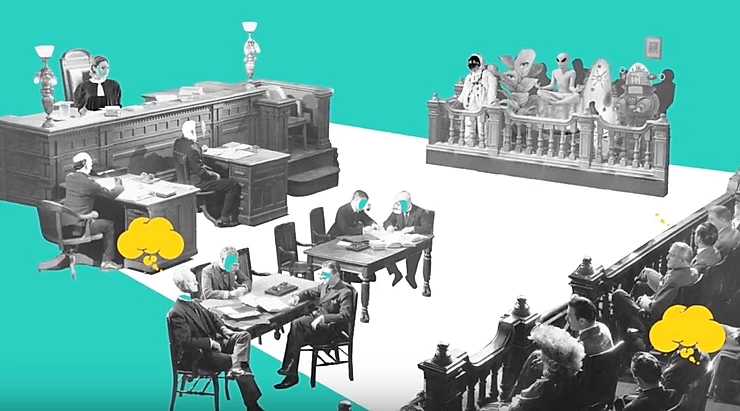
\includegraphics[height=\paperheight]{tribunal.png}}
%\section{\noindent\colorbox{shadecolor}
%	{\parbox{\dimexpr\textwidth-2\fboxsep\relax}{\textcolor{white}{Questions}}}}
%\usebackgroundtemplate{}

%-=-=-=-=-=-=-=-=-=-=-=-=-=-=-=-=-=-=-=-=-=-=-=-=
%	References:
%-=-=-=-=-=-=-=-=-=-=-=-=-=-=-=-=-=-=-=-=-=-=-=-=
\begin{frame}[t,allowframebreaks]{References}
\tiny
\bibliographystyle{apalike}
\bibliography{references}	
\end{frame}

\end{document}
